\chapter{Implementacja}
W niniejszym rozdziale przedstawiono szczegółową analizę implementacji dwuwymiarowej gry zręcznościowej z gatunku bijatyk. Omówienie obejmuje kluczowe aspekty techniczne projektu, takie jak tworzenie animacji, struktura klas, wzorce projektowe oraz implementacja mechanik gry, zarówno w trybie offline, jak i online. Szczególny nacisk położono na takie elementy, jak zarządzanie postaciami, detekcja kolizji, obsługa sieci oraz interfejs użytkownika, które razem stanowią rdzeń funkcjonalności i grywalności projektu.
\section{Tworzenie animacji}
Na rysunku \ref{fig:animacja} pokazano proces tworzenia animacji.
\begin{figure}
	\centering
		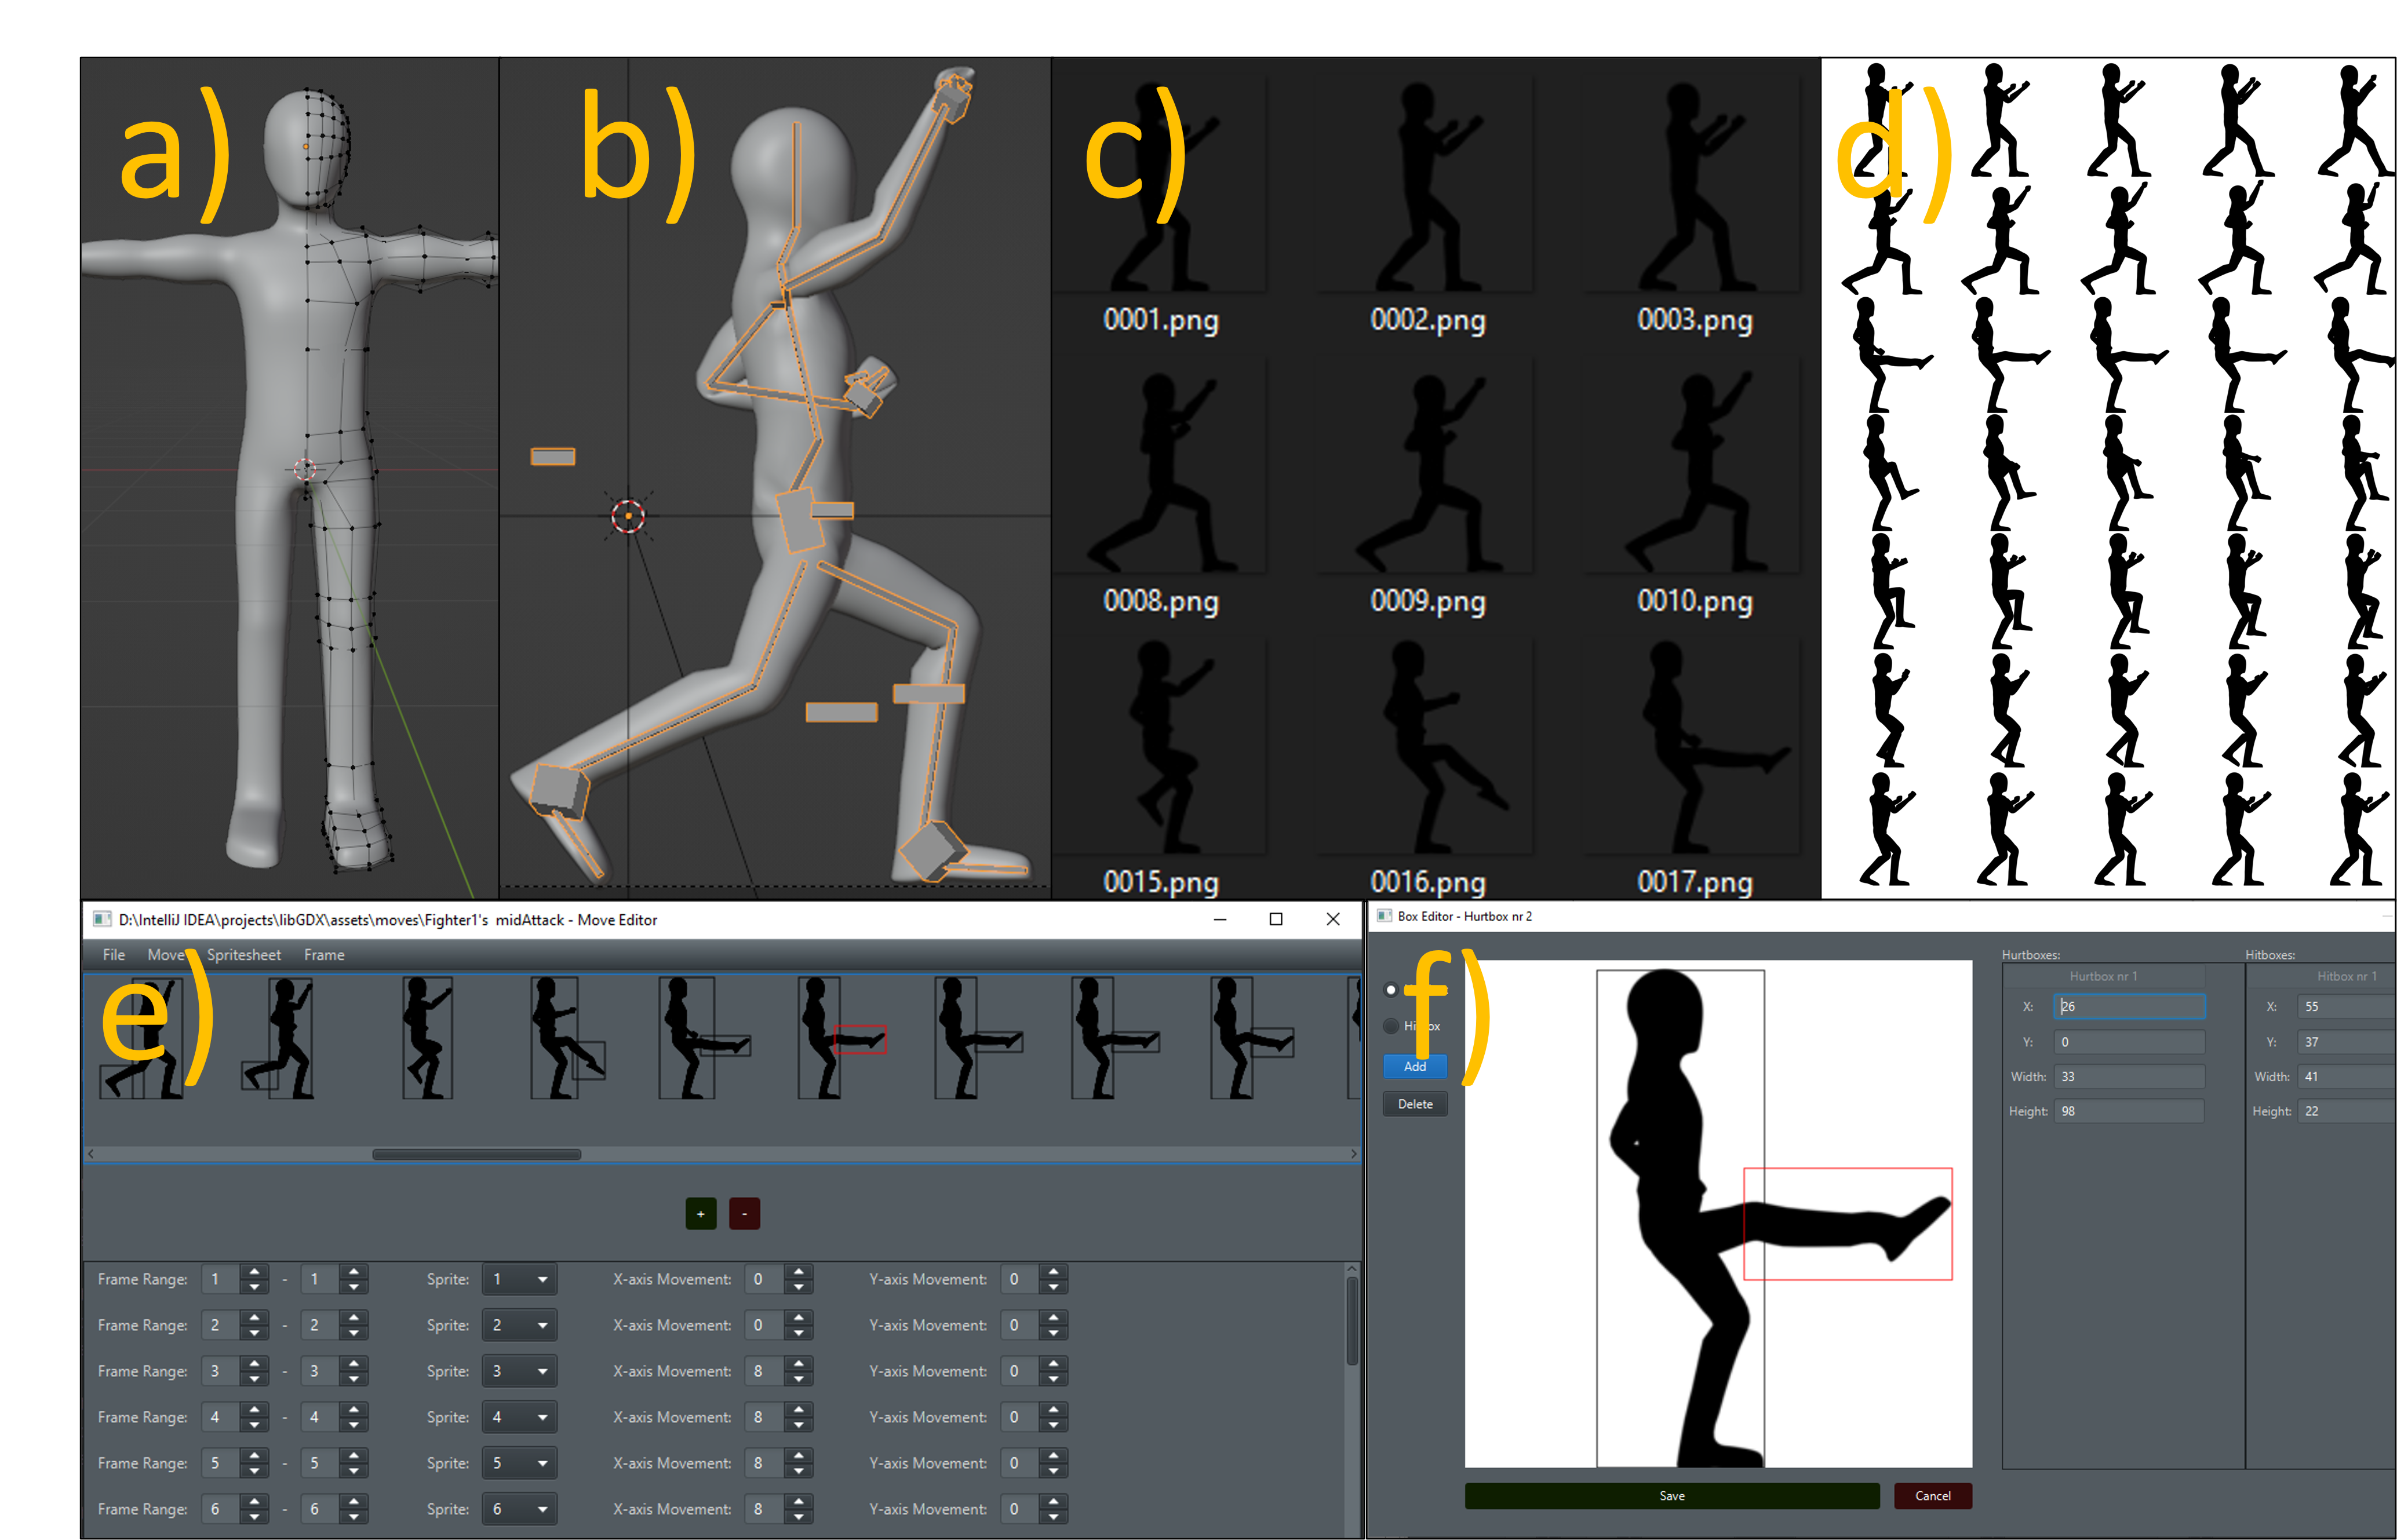
\includegraphics[width=0.64\linewidth]{rys03/animacja}
	\caption{Proces tworzenia animacji: a) modelowanie, b) \emph{rigging}, c) wygenerowanie \emph{sprite'ów}, d) stworzenie \emph{spritesheet'a}, e) edycja klatek, f) definicja \emph{hurtbox'ów} i \emph{hitbox'ów}}
	\label{fig:animacja}
\end{figure}
Na początku postać została zamodelowana w 3D. Użyto do tego narzędzia Blender. Następnie przeprowadzono \emph{rigging}, czyli proces dodawania szkieletu do modelu 3D, który pozwala na animowanie poszczególnych części ciała. Po ustawieniu postaci w pożądanych pozach, każda klatka animacji była renderowana i zapisywana jako seria oddzielnych plików graficznych (\emph{sprite'ów}). Te obrazy stanowiły podstawę dla każdego ruchu postaci w grze. Następnie używając narzędzia ImageMagick \emph{sprite'y} zostały połączone w jeden większy obraz zwany \emph{spritesheet'em}. Używając stworzonego przez autora pracy, na potrzeby tego projektu, narzędzia do edycji animacji Move Editor, stworzono wpisy do każdej klatki, opisujące między innymi ruch postaci. W Move Editorze określano również \emph{hurtbox'y} i \emph{hitbox'y} dla każdej klatki animacji. \emph{Hurtbox} to obszar, w którym postać może otrzymać obrażenia, natomiast \emph{hitbox} to obszar, w którym postać zadaje obrażenia. Ta funkcjonalność jest kluczowa dla mechaniki gry, ponieważ decyduje o tym, kiedy ataki postaci trafiają lub są blokowane. Po zakończeniu edycji \emph{spritesheet} wraz z opisem klatek w formacie json zostały zapisane w odpowiedniej strukturze plików, aby mogły być bezpośrednio wykorzystane w grze. Oprócz animacji samych postaci została również wykonana animacja zachodzącego słońca, która następnie została wykorzystana do stworzenia dynamicznego tła wyświetlającego się podczas rozgrywki.


\section{Struktura klas}
Na rysunku \ref{fig:struktura_klas} przedstawiono główne klasy stworzone na potrzeby gry. W poniższych podsekcjach zamieszczono krótki opis każdej z nich.
\begin{figure}[htb]
	\centering
		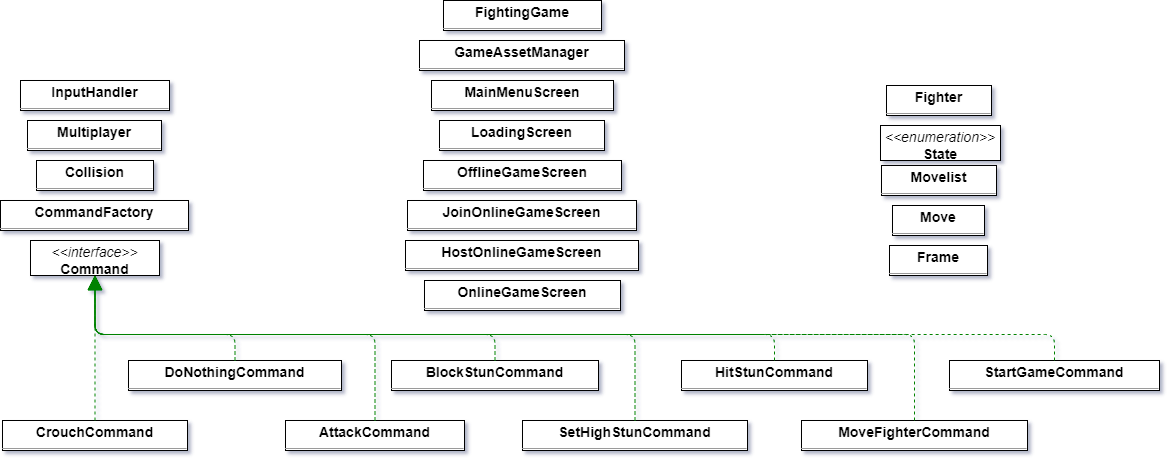
\includegraphics[width=1\linewidth]{rys03/struktura_klas}
	\caption{Struktura zaprojektowanych klas}
	\label{fig:struktura_klas}
\end{figure}

\subsection{Główna struktura gry}
\texttt{FightingGame} służy jako centrum zarządzania głównymi aspektami gry, takimi jak inicjalizacja, cykl życia gry oraz przełączanie pomiędzy różnymi ekranami (np. menu, gra itp.). W~procesie inicjalizacji wykorzystuje klasę \texttt{GameAssetManager}, która odpowiada za wczytywanie i~zarządzanie zasobami gry, takimi jak tekstury, dźwięki i~inne elementy multimedialne.

\texttt{MainMenuScreen}, \texttt{LoadingScreen}, \texttt{OfflineGameScreen}, \texttt{JoinOnlineGameScreen}, \texttt{HostOnlineGameScreen} oraz \texttt{OnlineGameScreen} są klasami reprezentującymi różne ekrany w grze, każdy z nich implementuje interfejs \texttt{Screen} dostarczony przez framework \texttt{libGDX}. Zapewniają one różnorodne interfejsy uzytkownika i są odpowiedzialne za prezentację odpowiedniego widoku w zależności od stanu gry.

\subsection{Mechanika rozgrywki}
Klasa \texttt{Fighter} reprezentuje postać walczącą. Przechowuje ona wartości takie jak zdrowie, pozycję, \emph{hurtbox'y} i \emph{hitbox'y} postaci oraz stan w którym aktualnie się znajduje. Ten stan reprezentowany jest przez typ wyliczeniowy \texttt{State} i obejmuje takie sytuacje jak ,,chodzenie do przodu'', ,,cofanie się'', ,,kucanie'' jak i wykonywanie różnych ataków albo otrzymywanie ich na bloku lub bez niego. Na podstawie tej klasy często wykonuje się logika reszty programu. 

Awatar, którym steruje gracz, posiada zestaw ruchów zawarty w klasie \texttt{Movelist}. Ta klasa przetrzymuje poszczególne ruchy o klasie \texttt{Move}. Każdy cios jest opisany poprzez pojedyncze klatki za pomocą klasy \texttt{Frame}, w których znajduje się informacja o ruchu jaki postać ma wykonać, jaki zestaw obszarów określających kolizję ma mieć wpływ na postać w danym momencie oraz jaki \texttt{sprite} ma zostać wyświetlony.

\subsection{Wykrywanie kolizji, obsługa wejścia i wzorzec \emph{command}}
Klasy \texttt{Command}, \texttt{CommandFactory}, \texttt{DoNothingCommand}, \texttt{BlockStunCommand}, \texttt{HitStunCommand}, \texttt{SetHighStunCommand}, \texttt{MoveFighterCommand}, \texttt{StartGameCommand} wdrażają wzorzec programowania \emph{command} (polecenia, \cite{GPP}), umożliwiając abstrakcyjne reprezentacje akcji, które mogą być wykonane w grze. \texttt{Command} jest interfejsem dla wszystkich komend, \texttt{CommandFactory} jest fabryką do tworzenia instancji komend, a pozostałe klasy są konkretnymi komendami, które mogą być wywołane przez graczy lub system gry. Klasa \texttt{InputHandler} zajmuje się obsługą wejścia od użytkownika - tworzy komendy na podstawie przycisku naciśniętego przez gracza oraz aktualnego stanu postaci. \texttt{Collision} zarządza detekcją kolizji między postaciami w grze oraz wpływa na stan tych postaci. \texttt{Multiplayer} odpowiada za implementację funkcjonalności sieciowych, umożliwiając grę wieloosobową poprzez zarządzanie połączeniami i komunikacją między graczami. Gdy postać jest sterowana przez gracza połączonego przez internet to właśnie ta klasa podaje komendy do wykonania przez jego awatar wpływając na działanie \texttt{InputHandler'a}.

\section{Fragmenty kodu}
W tej sekcji zostaną omówione fragmenty kodu, które zostały uznane przez autora pracy inżynierskiej za kluczowe w działaniu programu.
\subsection{Interfejs \texttt{Command}}
Na listingu \ref{list:command} zaprezentowano interfejs, który jest implementowany przez wiele innych klas. Interfejs ten nakazuje implementującym go klasom stworzenie metody \texttt{execute}, która najczęściej zmieniać ma stan jakiegoś obiektu (np.\ z klasy \texttt{Fighter}) oraz metody \texttt{undo}, mającej za zadanie wycofanie zmian wprowadzonych metodą \texttt{execute}. Dzięki temu podejściu można na przykład łatwo zmieniać przypisane do przycisków zadania lub stworzyć historię wciśniętych przycisków, a także system powtórek bazujących na logice \emph{undo}. Dodatkowo, tworzenie obiektów reprezentujących wykonywane akcje ułatwia proces tworzenia kodu sieciowego.
\begin{lstlisting}[language=Java,style=JavaStyle,label=list:command,caption=Interfejs \texttt{Command},
                   basicstyle=\footnotesize\ttfamily]
public interface Command {
    void execute(Entity entity);
    void undo(Entity entity);
}
\end{lstlisting}

\subsection{Klasa \texttt{Fighter}}
Klasa \texttt{Fighter} zarządza stanem i zachowaniem postaci w grze. Zawiera informacje o zdrowiu, listy obszarów trafień (\emph{hitboxes}) i obszarów, które mogą zostać trafione (\emph{hurtboxes}), oraz zestaw ruchów (\emph{movelist}). Wykorzystuje ona wzorzec programowania \emph{update}. Sprowadza się on do implementacji metody aktualizacji stanu, która symuluje jedną klatkę zachowania obiektu. Na listingu \ref{list:fighter} można zauważyć, że metoda ta tworzy rozkaz za pomocą klasy \texttt{InputHandler}, a~następnie wykonuje go. W kolejnym kroku, jeżeli gracz uczestniczy w rozgrywce online, jego komenda jest przesyłana do drugiego gracza z pomocą klasy \texttt{Multiplayer}. Na końcu postać w grze aktualizuje wyświetlany \texttt{sprite} oraz inne informacje dotyczące aktualnej klatki animacji.

\begin{lstlisting}[language=Java,style=JavaStyle,label=list:fighter,caption=Funkcja update w klasie Fighter,
                   basicstyle=\footnotesize\ttfamily]
public void update() {
    Command command = inputHandler.handleInput();
    command.execute(this);
    if (multiplayer != null && (player == Player.PLAYER1 || player == Player.PLAYER2)) {
        multiplayer.sendCommand(command);
    }
    updateAnimation();
}
\end{lstlisting}

\subsection{Klasa \texttt{OfflineGameScreen}}
Listing \ref{list:offline_game} przedstawia implementację klasy \texttt{OfflineGameScreen}. Klasa ta wykorzystuje wzorzec pętli gry (\emph{game loop pattern}), wraz z wzorcem aktualizacji (\emph{update pattern}), aby zarządzać cyklem życia gry w trybie \emph{offline}. Konstruktor inicjalizuje stan gry, przydzielając graczy i tworząc kolekcję bytów (\texttt{entities}), które będą aktualizowane i renderowane w każdym cyklu gry. Inicjalizuje również system kolizji, który jest odpowiedzialny za wykrywanie i rozwiązywanie interakcji między bytami. Klasa implementuje interfejs \texttt{Screen} z frameworka \texttt{LibGDX}, co oznacza, że musi dostarczyć implementację metody \texttt{render}, która jest wywoływana na każdą klatkę gry. Ta metoda jest rdzeniem pętli gry. Przyjmuje parametr \texttt{delta}, który reprezentuje czas, jaki upłynął od ostatniej klatki, umożliwiając aktualizacje oparte na czasie rzeczywistym. Na początku każdej klatki ekran jest czyszczony. 

Metoda \texttt{updateEntities} jest wywoływana w celu zaktualizowania stanu wszystkich bytów w grze. Zawiera logikę warunkową, która decyduje, czy byty powinny być aktualizowane w stanie bezczynności (\texttt{idle}), po zakończeniu rundy (\texttt{updateRoundEnd}), czy w standardowym trybie gry, gdzie każdy byt jest aktualizowany poprzez wywołanie jego metody update. Te dwie pierwsze są oddzielone od standardowego trybu ze względu na to że w trybie online będą one mogły wykonywać się po stronie klienta, niezależnie od przychodzących przez internet informacji od drugiego gracza. Po zaktualizowaniu bytów, system kolizji jest aktualizowany, aby sprawdzić i przetworzyć wszelkie kolizje, które miały miejsce pomiędzy bytami. 

Na koniec metoda \texttt{renderGame} odpowiada za narysowanie aktualnego stanu gry na ekranie.

\begin{lstlisting}[language=Java,style=JavaStyle,label=list:offline_game,caption=Klasa \texttt{OfflineGameScreen},
                   basicstyle=\footnotesize\ttfamily]
public class OfflineGameScreen implements Screen {
    FightingGame game;
    private Collection<Entity> entities;
    private Collision collision;
    ...// Pozostałe tekstury, dźwięki itp

    public OfflineGameScreen(FightingGame game) {
        // Przydzielanie graczy
        game.player1.setPlayer(Player.PLAYER1);
        game.player2.setPlayer(Player.PLAYER2);

        // Inicjalizacja kolekcji bytów i kolizji
        entities = new ArrayList<>();
        entities.add(game.player1);
        entities.add(game.player2);
        collision = new Collision(game.player1, game.player2); 
        ...// Pobieranie załadowanych zasobów za pomocą AssetManagera
    }

    @Override
    public void render(float delta) {
        ...
        //clear
        clearScreen();
        //update
        updateEntities();
        //render
        renderGame();
		...
    }
		
		private void updateEntities() {
        if (isCountdownActive || isFightMessageActive) {
            game.player1.updateIdle();
            game.player2.updateIdle();
        } else if (isWinnerMessageActive) {
            game.player1.updateRoundEnd();
            game.player2.updateRoundEnd();
        } else {
            for (Entity entity : entities) {
                entity.update();
            }
            collision.update();
        }
    }
		...
}
\end{lstlisting}

\subsection{Klasa \texttt{Multiplayer}}
Klasa \texttt{Multiplayer} została stworzona w celu obsługi połączenia między graczami w trybie online. Wykorzystuje ona biblioteki kryo \cite{Kryo}, kryonet \cite{Kryonet} oraz weupnp \cite{weupnp}, co jest widoczne w~importach klasy w listingu \ref{list:multiplayer}. Konstruktor klasy nie otwiera jeszcze żadnego połączenia, a~konkretne metody obsługi połączenia są wywoływane dopiero po wybraniu przez użytkownika odpowiedniego trybu gry. 

Jeśli gracz wybierze opcję hostowania meczu, oznacza to uruchomienie serwera na jego komputerze za pomocą funkcji \texttt{initializeServer}. Funkcja ta rozpoczyna od znalezienia wolnego portu, którym domyślnie jest port 54555. Następnie próbuje otworzyć go za pomocą funkcji \texttt{openPortUPnP}, która wyszukuje dostępny router i sprawdza jego zewnętrzny adres IP, a następnie tworzy mapowanie portów. Po tych krokach tworzony jest serwer i przypisywane są do niego klasy do serializacji i deserializacji. Serwer nasłuchuje różne zdarzenia, takie jak połączenie i rozłączenie drugiego gracza, które zmieniają flagi klasy \texttt{Multiplayer}. Dodatkowo, jeśli do serwera przyjdzie instancja obiektu \texttt{Command} jest ona dodawana do kolejki komend. Na podstawie tej kolejki \texttt{InputHandler} definiuje zachowanie postaci gracza połączonego przez sieć. Ostatecznie serwer jest przypisywany do portu, na którym ma pracować. 

W~przypadku wyboru przez użytkownika opcji dołączenia do pokoju i podania kodu uzyskanego od drugiego gracza, uruchamiana jest funkcja \texttt{initializeClient}. Podobnie jak w~przypadku serwera, klient również nasłuchuje przychodzące wiadomości. Jedyną różnicą jest obsługa konkretnych komend, takich jak rozpoczęcie gry czy wiadomość o powaleniu przeciwnika. Reszta komend jest obsługiwana w podobny sposób jak na serwerze. 

Klasa \texttt{Multiplayer} posiada także funkcje do zamykania serwera i klienta \texttt{closeServer} i~\texttt{closeClient}, które służą do zakończenie połączenia po zakończeniu rozgrywki i w przypadku serwera również zakończenie przekierowania portów na routerze.

\begin{lstlisting}[language=Java,style=JavaStyle,label=list:multiplayer,caption=Klasa \texttt{Multiplayer},
                   basicstyle=\footnotesize\ttfamily]
package com.mygdx.game;

import com.esotericsoftware.kryo.Kryo;
import com.esotericsoftware.kryonet.Connection;
import com.esotericsoftware.kryonet.Listener;
import com.esotericsoftware.kryonet.Server;
import com.esotericsoftware.kryonet.Client;
...
import org.bitlet.weupnp.GatewayDevice;
import org.bitlet.weupnp.GatewayDiscover;
import org.bitlet.weupnp.PortMappingEntry;


public class Multiplayer {
    private Server server;
    private Client client;
    private int serverPort;
    private int connectedPort;
    private boolean isAttemptingConnection = false;
    private boolean isConnected = false;
    private boolean startGame = false;
    private String lastErrorMessage = null;
	...
    String ipAddress;
    LinkedBlockingDeque<Command> commandQueue;

    public Multiplayer() {
        this.commandQueue = new LinkedBlockingDeque<>();
    }

    public void initializeServer() {
        isAttemptingConnection = true;
        serverPort = findFreePort();
        if (openPortUPnP(serverPort)) {
            System.out.println("UPnP: Port został otwarty");
        } else {
            System.out.println("UPnP: Nie udało się otworzyć portu, sprawdź konfigurację routera lub ustawienia firewalla");
        }
        server = new Server();
        client = null;
        configureKryo(server.getKryo());

        server.addListener(new Listener() {
            @Override
            public void connected(Connection connection) {
                isConnected = true;
                lastErrorMessage = null;
            }
            @Override
            public void received(Connection connection, Object object) {
                if (object instanceof Command) {
                    System.out.println("received: " + object);
                    handleCommand((Command) object);
                }
            }
            @Override
            public void disconnected(Connection connection) {
                isConnected = false;
                lastErrorMessage = "Disconnected";
            }
        });

        ipAddress = getPublicIpAddress();
        System.out.println("IpAddress: " + ipAddress);
        try {
            server.bind(serverPort);
            server.start();
            System.out.println(" Server started on serverPort: " + serverPort);
        } catch (IOException e) {
            lastErrorMessage = "Connection error: " + e.getMessage();
            e.printStackTrace();
        }
    }

    public void closeServer() {
        if (server != null) {
            server.stop();
            server = null;
            removePortUPnP(serverPort);
            System.out.println("Serwer zostal zamkniety.");
        }
    }


    public void initializeClient(String ipAddress, int port) {
        isAttemptingConnection = true;
        client = new Client();
        configureKryo(client.getKryo());

        client.addListener(new Listener() {
            @Override
            public void connected(Connection connection) {
                isConnected = true;
                lastErrorMessage = null;
            }
            @Override
            public void received(Connection connection, Object object) {
                if (object instanceof SetHighStunCommand) {
                    System.out.println("received: " + object);
                    player1IsHitStunned = true;
                }
                else if (object instanceof StartGameCommand) {
                    startGame = true;
                } else if (object instanceof Command) {
                    System.out.println("received: " + object);
                    handleCommand((Command) object);
                }
            }
            @Override
            public void disconnected(Connection connection) {
                isConnected = false;
                lastErrorMessage = "disconnected";
            }
        });

        try {
            client.start();
            //System.out.println("Klient probuje sie polaczyc z " + ipAddress + "/" + port);
            client.connect(5000, ipAddress, port);
            this.ipAddress = ipAddress;
        } catch (IOException e) {
            lastErrorMessage = "Connection error: " + e.getMessage();
            e.printStackTrace();
        }
    }

    public void closeClient() {
        if (client != null) {
            client.stop();
            client = null;
            System.out.println("Klient zostal zamkniety.");
        }
    }

    public void stopServer() {
        if (server != null) {
            // Usuń mapowanie portów za pomocą UPnP
            removePortUPnP(serverPort);
            server.stop();
            server.close();
            System.out.println("Serwer zatrzymany");
        }
    }

    private void handleCommand(Command command) {
        commandQueue.add(command);
    }

    public void sendCommand(Command command) {
        if (server != null) {
            System.out.println("send: " + command);
            server.sendToAllTCP(command);
        } else if (client != null) {
            System.out.println("send: " + command);
            client.sendTCP(command);
        }

    }

    public boolean openPortUPnP(int port) {
        try {
            GatewayDiscover discover = new GatewayDiscover();
            discover.discover();
            GatewayDevice d = discover.getValidGateway();

            if (d == null) {
                System.out.println("Nie znaleziono bramy UPnP!");
                return false;
            }

            System.out.println("Znaleziono brame UPnP: " + d.getModelName());

            // Pobierz zewnętrzny adres IP
            String externalIPAddress = d.getExternalIPAddress();
            System.out.println("Zewnetrzny adres IP to: " + externalIPAddress);

            // Utwórz mapowanie portów
            boolean done = d.addPortMapping(port, port, d.getLocalAddress().getHostAddress(), "TCP", "KryoNet Game Server");

            if (done) {
                System.out.println("Port przekierowany: " + port);
                return true;
            } else {
                System.out.println("Nie udalo się przekierować portu: " + port);
                return false;
            }
        } catch (Exception e) {
            e.printStackTrace();
            return false;
        }
    }

    public boolean removePortUPnP(int port) {
        try {
            GatewayDiscover discover = new GatewayDiscover();
            discover.discover();
            GatewayDevice d = discover.getValidGateway();
            if (d != null) {
                return d.deletePortMapping(port, "TCP");
            }
        } catch (Exception e) {
            e.printStackTrace();
        }
        return false;
    }
		...
}
									
\end{lstlisting}